% Recommended preamble:
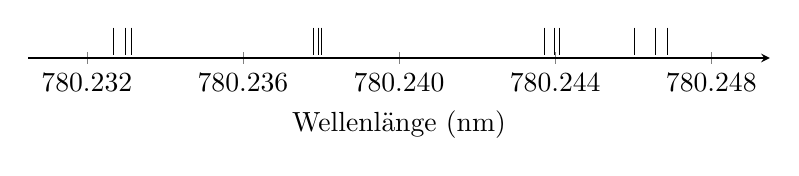
\begin{tikzpicture}
\begin{axis}[xmin={780.2305}, xmax={780.2495}, width={110mm}, height={20mm}, axis x line={bottom}, axis y line={none}, xlabel={Wellenlänge (nm)}, xtick={780.232,780.236,780.24,780.2439999999999,780.2479999999999}, scaled ticks={false}, x tick label style={/pgf/number format/.cd, fixed zerofill, 1000 sep={{ \, }}, precision={3}, /tikz/.cd}]
    \addplot[mark={|}, mark size={5pt}, only marks]
        table[row sep={\\}]
        {
            \\
            780.2331487748982  1.0  \\
            780.2330021440468  1.0  \\
            780.2468808430355  1.0  \\
            780.2326835201284  1.0  \\
            780.2465622077816  1.0  \\
            780.2460208472648  1.0  \\
            780.2380021521406  1.0  \\
            780.2379425162327  1.0  \\
            780.2441069857716  1.0  \\
            780.2378137847006  1.0  \\
            780.2439782522051  1.0  \\
            780.2437332880502  1.0  \\
        }
        ;
\end{axis}
\end{tikzpicture}
